% Chapter Template

\chapter{Oprogramowanie kwadrokoptera} % Main chapter title

\label{Chapter6} % Change X to a consecutive number; for referencing this chapter elsewhere, use \ref{ChapterX}

\lhead{Rozdział 6. \emph{Oprogramowanie}} % Change X to a consecutive number; this is for the header on each page - perhaps a shortened title

%----------------------------------------------------------------------------------------
%	SECTION 1
%----------------------------------------------------------------------------------------
\section{Struktura oprogramowania}

\begin{figure}[H]
	\centering
	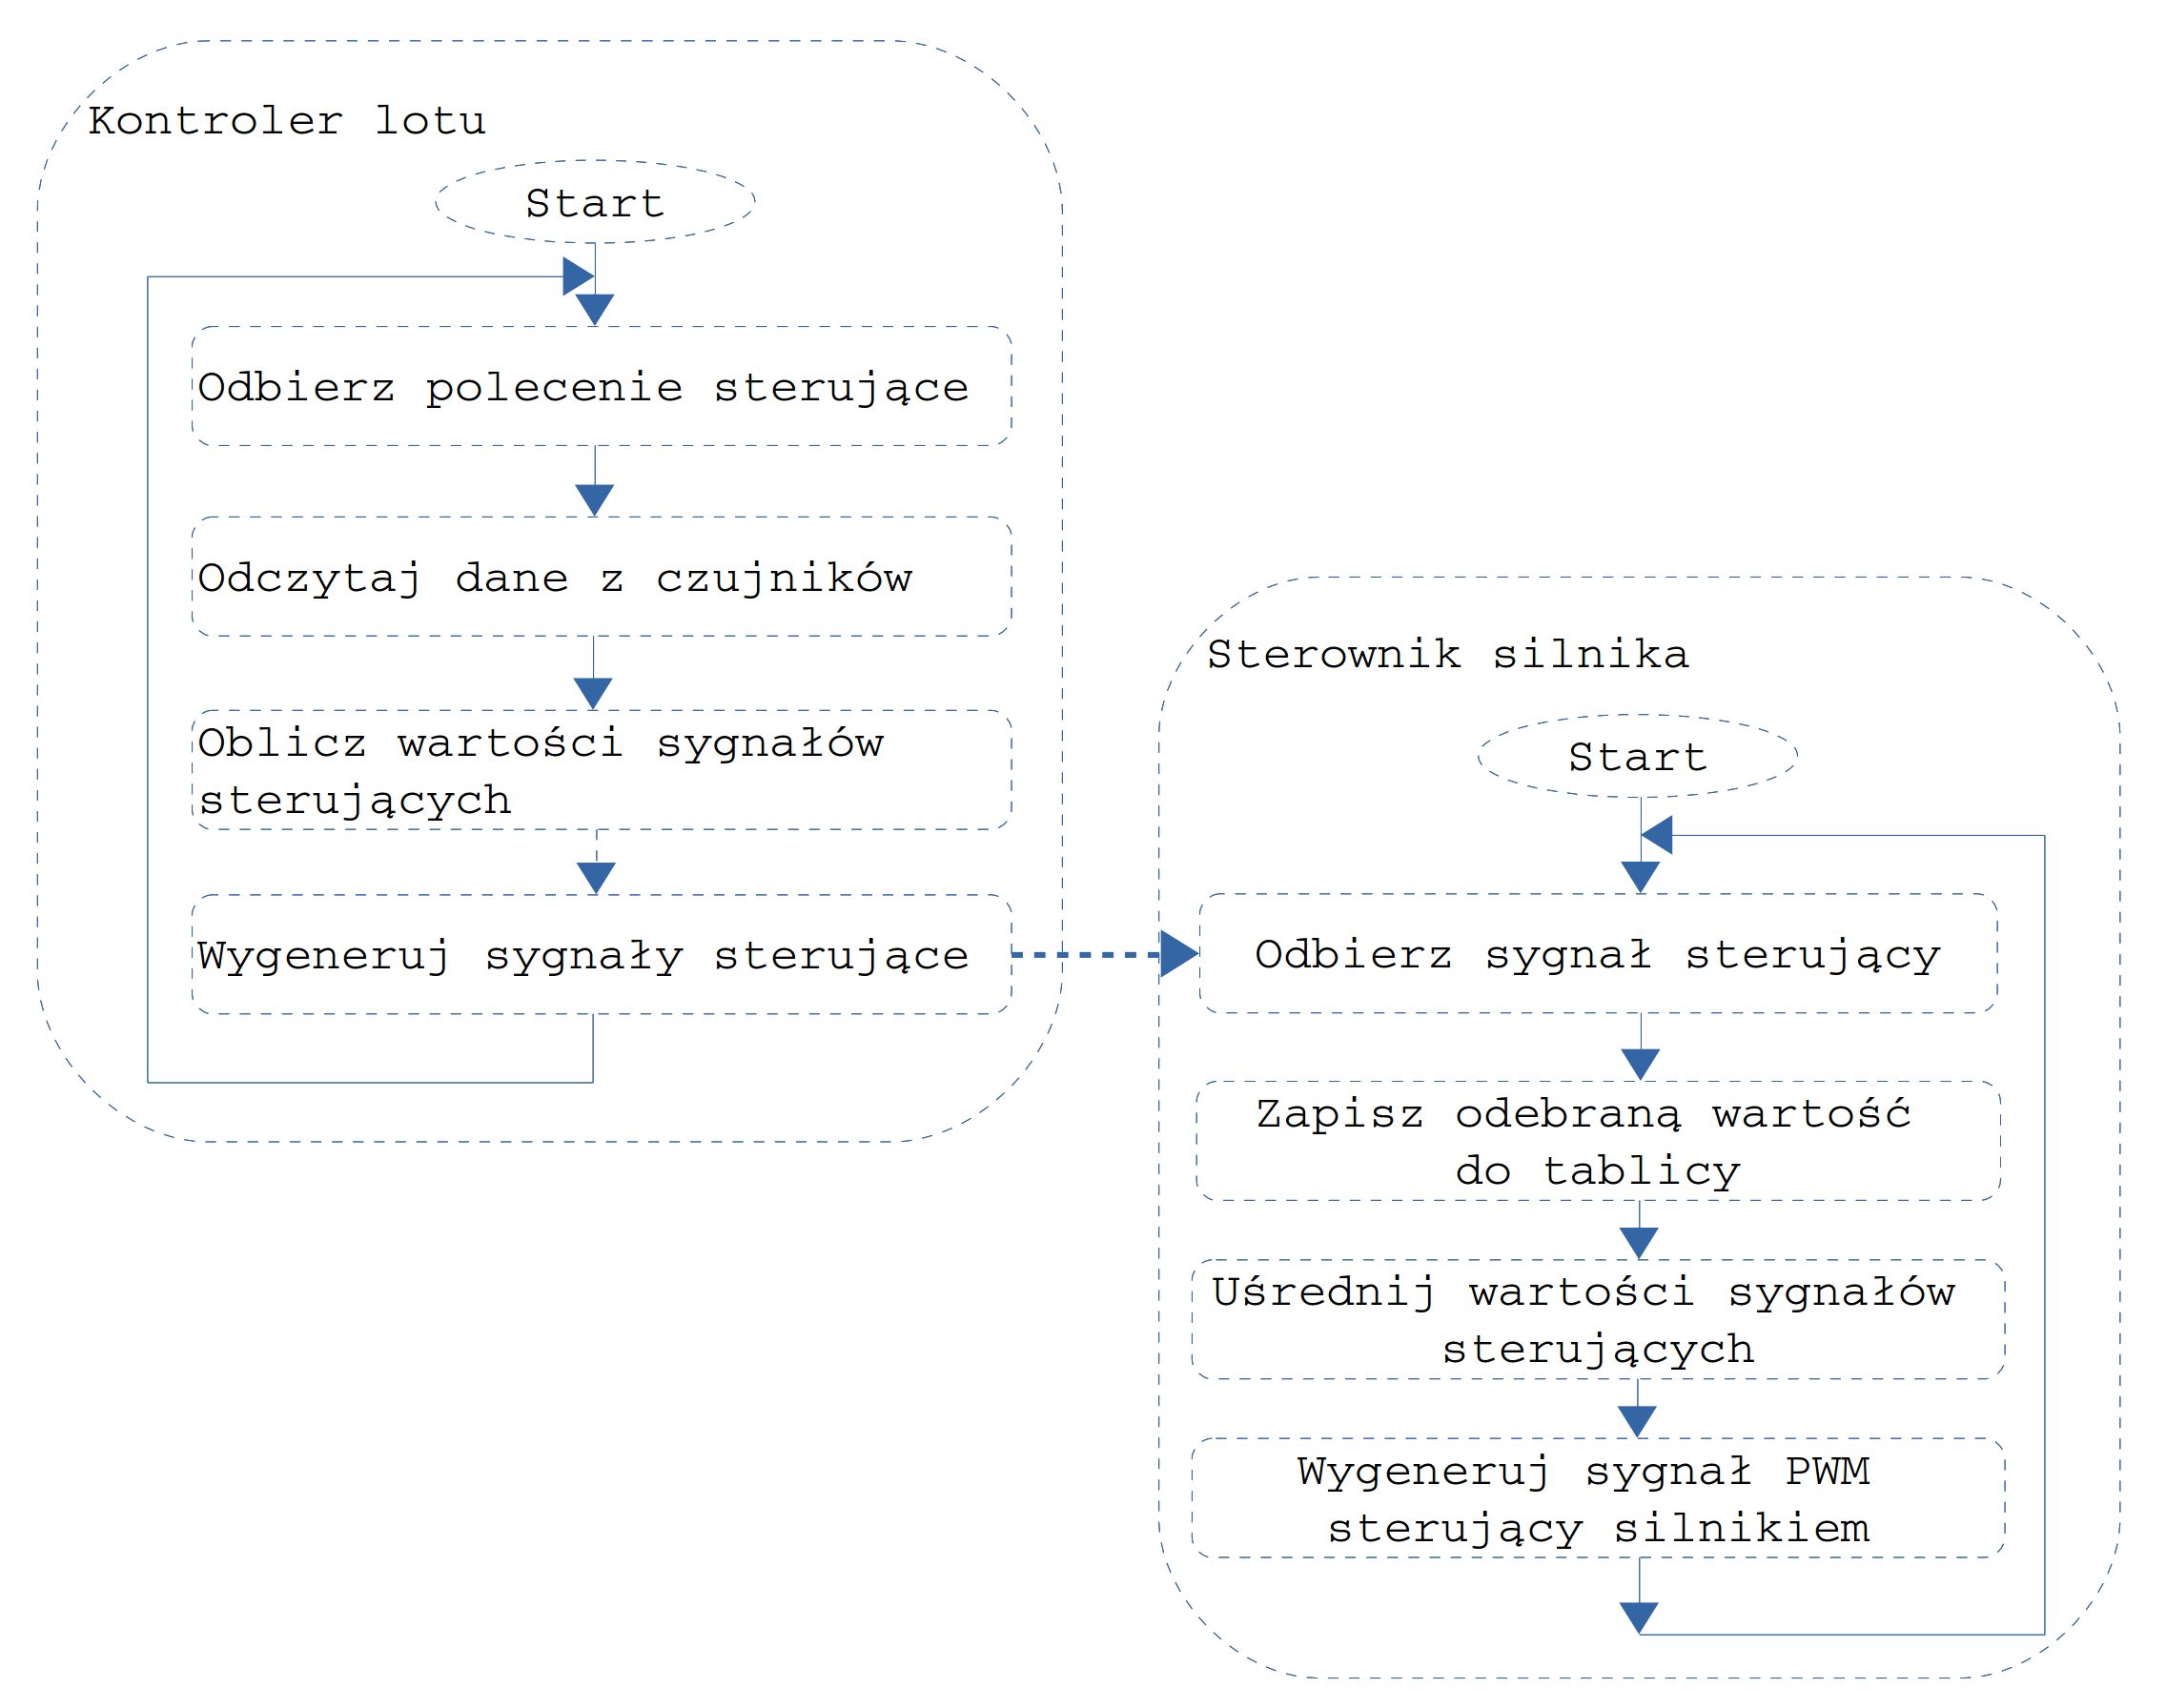
\includegraphics[width=1\textwidth]{Pictures/Struktura_oprogramowania.png}
		%\rule{35em}{0.5pt}
		\caption[Struktura oprogramowania kontrolera lotu oraz sterownika silnika]{Struktura oprogramowania kontrolera lotu oraz sterownika silnika}
	\label{fig:struktura_oprogramowania}
\end{figure}

Rysunek~\ref{fig:struktura_oprogramowania} przedstawia strukturę oprogramowania kontrolera lotu oraz sterownika silnika (dla uproszczenia na schemacie przedstawiony jest tylko jeden sterownik silnika). Pogrubioną strzałką łączącą bloki kontrolera lotu oraz sterownika silnika zaznaczono przesyłanie sygnałów sterujących generowanych przez kontroler lotu w przyjętym formacie modelarskim PWM opisanym w rozdziale~\ref{Chapter2}.

\section{Kontroler lotu}

\subsection{Funkcje programowe}

Oprogramowanie kontrolera lotu realizuje cztery podstawowe zadania:

\begin{itemize}
	\item Odbiór poleceń 
	\item Odczyt pomiarów z czujników
	\item Generowanie sygnałów sterujących 
	\item Wysyłanie sygnałów sterujących do kontrolerów silników
\end{itemize}

Pierwsza wersja oprogramowania powstała w języku assembler avr, jednakże zrezygnowano z tej koncepcji ze względu na dużą liczbę gotowych bibliotek służących do obsługi czujników pomiarowych, napisanych w języku C oraz ze względu na istotne trudności powstające przy programowaniu w assemblerze operacji arytmetycznych na liczbach 16-bitowych oraz 32-bitowych. Operacje te są wykonywane przez algorytm stabilizacji lotu. 

Druga, finalna wersja oprogramowania została napisana w języku C, z wykorzystaniem gotowych bibliotek służących do obsługi czujnika MPU-6050 oraz bibliotek implementujących regulator PID, w których autor pracy wprowadził poprawki adaptujące je do projektu kwadrokoptera.


\subsection{Komunikacja radiowa}

Komunikacja radiowa realizowana jest za pomocą modułu Bluetooth HC-06 (lub kompatybilnego HC-05) udostępniającego interfejs UART do nadawania i odbierania danych z poziomu mikrokontrolera sterującego kwadrokopterem.
Chcąc zrealizować płynną transmisję danych między kwadrokopterem a użytkownikiem obrano następujące założenia:
\begin{itemize}
	\item Kwadrokopter jest widziany z punktu użytkownika jako zbiór 8-bitowych rejestrów.
	\item Wartości rejestrów są kwadrokoptera przechowywane w pamięci RAM jako tablica zmiennych 8-bitowych.
	\item Protokół binarny służący do wymiany danych między użytkownikiem a kwadrokopterem ma poniższe cechy:
	\begin{itemize}
		\item minimum dwie komendy: zapis rejestrów i odczyt rejestrów,
		\item użytkownik zawsze inicjuje transmisję.
	\end{itemize} 
\end{itemize}

Idea zastosowania protokołu binarnego znacząco upraszcza implementację oprogramowania po stronie mikrokontrolera, skracając tym samym czas potrzebny na przetwarzanie danych. Struktura wiadomości wygląda następująco:

<Kod komendy><Długość wiadomości w bajtach><Pole danych wiadomości>

Pola ''Kod komendy'' oraz ''Długość wiadomości'' mają rozmiar jednego bajtu, pole danych wiadomości ma długość o dwa bajty mniejszą niż wartość wpisana w polu długości wiadomości.
Pole danych wiadomości może zawierać różną treść w zależności od kodu komendy. 
\begin{itemize}
	\item Komenda zapisu rejestrów - pole danych wiadomości ma długość co najmniej trzech bajtów
	\begin{itemize}
		\item Adres pierwszego rejestru do zapisu
		\item Liczba rejestrów do zapisu
		\item Pole zawierające wartości kolejnych zapisywanych rejestrów
	\end{itemize}
	\item Komenda odczytu rejestrów - pole danych wiadomości ma długość dwóch bajtów
	\begin{itemize}
		\item Adres pierwszego rejestru do odczytu
		\item Liczba rejestrów do odczytu
	\end{itemize} 	
\end{itemize} 

Poniższy listing przedstawia strukturę zdefiniowaną w programie, która jest używana do przechowywania danych odebranych  przez kwadrokopter.

\begin{lstlisting}
#define FRAME_DATA_BUFFER_SIZE 35
typedef struct
{
    union
    {
        struct
        {
            volatile uint8_t command;
            volatile uint8_t data_count;
            uint8_t data[FRAME_DATA_BUFFER_SIZE];
        } frame;
        uint8_t raw_data[2+FRAME_DATA_BUFFER_SIZE];
    };
    //Frame control signals
    volatile uint8_t data_ready;
    volatile uint8_t data_index;
}QuadrocopterData;
\end{lstlisting}

Składa się ona z tablicy ''raw\_data'' przechowującej dane bezpośrednio odebrane przez interfejs UART. Następnie za pomocą unii, dane z tablicy ''raw\_data'' rzutowane są na kod komendy, długość wiadomości oraz polę danych wiadomości.

Dodatkowo w skład struktury wchodzą dwie flagi:
\begin{itemize}
	\item data\_ready - flaga ustawiana w przerwaniu odbioru danych przez interfejs UART, informująca program główny o odebraniu całej wiadomości.
	\item data\_index - index wykorzystywany przez procedurę odbierającą dane przez interfejs UART do zapisywania danych w tablicy ''raw\_data''. 
\end{itemize}

Poniższy listing przedstawia procedurę inicjalizacji interfejsu UART. Składa się ona z wyzerowania pól struktury ''quadrocopter\_rx\_data'' przechowującej dane odebrane przez kwadrokopter oraz z inicjalizacji sprzętowego modułu UART, w który wyposażony jest mikrokontroler ATmega328p, poprzez ustawienie rejestrów:
\begin{itemize}
	\item UBRR0H, UBRR0L, UCSR0A - rejestry odpowiedzialne za konfigurację szybkości transmisji
	\item UCSR0C - rejetsr odpowiedzialny za ustawianie formatu ramki interfejsu UART
	\item UCSR0B - rejestr odpowiedzialny za włączanie nadajnika oraz osbiornika sprzętowego modułu UART oraz włączanie przerwania odbioru danych
\end{itemize}

\begin{lstlisting}
void UART_init(void)
{

    uint8_t index;
    for(index = 0; index < 18; index++)
    {
        quadrocopter_rx_data.raw_data[index] = index;
    }
    quadrocopter_rx_data.data_ready = 0;
    quadrocopter_rx_data.data_index = 0;
    quadrocopter_rx_data.frame.command = 0;
    quadrocopter_rx_data.frame.data_count = 1;

	//Set baud rate - 57600 baud rate + double speed mode
	UBRR0H = (uint8_t)(34>>8);
	UBRR0L = (uint8_t)(34);
	UCSR0A = (1<<U2X0);
	//Set frame format: 8data, No parity, 1stop bit
	UCSR0C = (3<<UCSZ00);
	//Enable receiver and transmitter
	UCSR0B = ((1<<RXCIE0)|(1<<RXEN0)|(1<<TXEN0));

}
\end{lstlisting}

Przedstawiony poniżej listing przedstawia deklaracje rejestrów wewnętrznych kwadrokoptera, widocznych z poziomu użytkownika. 

\begin{lstlisting}
#define REG_COUNT 35
uint8_t reg_array[REG_COUNT];// = {0};
typedef void (*handler)(void);
handler reg_update_handler_array[REG_COUNT];// = {0};

#define REG_STATUS 	0
#define REG_COMMAND 	1

#define REG_THRUST	2
#define REG_PITCH	3
#define REG_ROLL	4
#define REG_YAW		5

#define REG_PID_X_PH		6//-
#define REG_PID_X_PL		7//-
#define REG_PID_X_IH		8//-- PID X
#define REG_PID_X_IL		9//-- PID X
#define REG_PID_X_DH		10//-
#define REG_PID_X_DL		11//-

#define REG_PID_Y_PH		12//-
#define REG_PID_Y_PL		13//-
#define REG_PID_Y_IH		14//-- PID Y
#define REG_PID_Y_IL		15//-- PID Y
#define REG_PID_Y_DH		16//-
#define REG_PID_Y_DL		17//-

#define REG_PID_Z_PH		18//-
#define REG_PID_Z_PL		19//-
#define REG_PID_Z_IH		20//-- PID Z
#define REG_PID_Z_IL		21//-- PID Z
#define REG_PID_Z_DH		22//-
#define REG_PID_Z_DL		23//-

#define REG_LED			24

#define REG_FL_PWM		25
#define REG_FR_PWM		26
#define REG_BL_PWM		27
#define REG_BR_PWM		28

#define REG_FR_BL_ENABLE	29
#define REG_FL_BR_ENABLE	30

#define REG_GX_OFFSET		31
#define REG_GY_OFFSET		32
#define REG_GZ_OFFSET		33

#define REG_LOG1_ENABLE		34
\end{lstlisting}

Jak widać jest to tablica 8-bitowych zmiennych ''reg\_array'' o rozmiarze zdefiniowanym za pomocą makra ''REG\_COUNT''. Następnie zdefiniowane są nazwy kolejnych rejestrów wraz z przypisanymi do nich adresami. Funkcje poszczególnych rejestrów omówiono poniżej:
\begin{itemize}
	\item Adresy 0-1: Nieużywane rejestry, przewidziane na potrzeby rozszerzania funkcji protokołu w przyszłości.
	\item Adresy 2-5: Rejestry używane w trakcie lotu, przechowujące zadane wartości ciągu silników oraz prędkości kątowych wokół trzech osi.
	\item Adresy 6-11: Rejestry przechowujące 16-bitowe wartości współczynników P,I,D kontrolera PID, odpowiedzialnego za stabilizację prędkości kątowej wokół osi X.
	\item Adresy 12-17: Rejestry przechowujące 16-bitowe wartości współczynników P,I,D kontrolera PID, odpowiedzialnego za stabilizację prędkości kątowej wokół osi Y.
	\item Adresy 18-23: Rejestry przechowujące 16-bitowe wartości współczynników P,I,D kontrolera PID, odpowiedzialnego za stabilizację prędkości kątowej wokół osi Z.
	\item Adres 24: Rejestr używany do testów, włączający debugowe diody LED na płytce kontrolera lotu.
	\item Adresy 25-28: Rejestry używane do testów, służące do wpisania bezpośredniej wartości sygnałów PWM wysyłanych do odpowiedniego kontrolera silnika.
	\item Adresy 29-30: Rejestry używane do testów, służące do włączania testowania regulatora PID dla osi X lub Y.
	\item Adresy 31-33: Rejestry używane do programowego wprowadzania offsetu dla wartości odczytywanych z żyroskopu.
	\item Adres 34: Rejestr używany do testów, służący do włączania wysyłania komunikatów debugowych z programu.
\end{itemize}

Oprócz tablicy przechowującej wartości rejestrów wewnętrznych kwadrokoptera, w kodzie programu zdefiniowana jest również tablica wskaźników na funkcje, które są wołane przy modyfikacji wartości odpowiadającego im rejestru wewnętrznego kwadrokoptera. Jest to bardzo proste i pożyteczne narzędzie, dające możliwość automatycznego wywoływania odpowiednich funkcji przy modyfikacji wybranych rejestrów.


Poniższy listing przedstawia funkcję służącą do zapisu rejestrów kwadrokoptera. Jako parametry wejściowe przyjmuje ona rozmiar całej odebranej ramki danych wyrażony w bajtach, oraz wskaźnik na pole danych wiadomości.

\begin{lstlisting}
#define INVALID_DATA_COUNT -2
#define INVALID_REG_ADDRESS -3
int8_t reg_write_command(uint8_t data_count, uint8_t *data)
{
	uint8_t reg_address;
	uint8_t reg_count;
	uint8_t *reg_values;
	reg_address = data[0];
	reg_count = data_count -1;
	reg_values = data+1;

	if(0 == reg_count)
	{
		return INVALID_DATA_COUNT;
	}
	if(REG_COUNT <=  reg_address)
	{
		return INVALID_REG_ADDRESS;
	}
	uint8_t index;
	uint8_t ret;
	ret = 0;
	for(index = 0; ((index < reg_count) && ((reg_address + index) < REG_COUNT));index++)
	{
		uint8_t temp;
		temp = reg_address + index;
		UART_print_s("[Addr: ");
		UART_print_d(&temp,UINT_8);
		temp = reg_values[index];
		UART_print_s(" Value: ");
		UART_print_d(&temp,UINT_8);
		UART_print_s("]");
		UART_println();
		reg_array[reg_address+index] = reg_values[index];
		if(0 != reg_update_handler_array[reg_address+index])
		{

			UART_print_s("Running register update handler");
			UART_println();
			reg_update_handler_array[reg_address+index]();
		}
		ret++;
	} 
	return ret;
}
\end{lstlisting}

Zapis rejestrów odbywa się w dwóch krokach:

Sprawdzanie prawidłowości odebranych danych: funkcja sprawdza czy pola odpowiadające liczbie rejestrów do zapisu oraz adresu pierwszego rejestru do zapisu mają prawidłowe wartości.

Zapis rejestrów: funkcja przechodzi po kolejnych indeksach tablicy przechowującej wartości rejestrów kwadrokoptera, i zastępuje je nowymi wartościami pobieranymi z pola danych wiadomości. Jednocześnie przy każdym zapisie rejestru funkcja sprawdza, czy w tablicy reg\_update\_handler\_array znajduje się wskaźnik na funkcję, która ma zostać wywołana podczas zmiany jego wartości. Jeśli pole w tablicy nie ma wartości 0, następuje wywołanie procedury przypisanej do modyfikowanego rejestru.

Działanie funkcji odczytującej wartości rejestrów kwadrokoptera jest analogiczne, dlatego też zbędne jest omawianie kodu tej funkcji.

Wykorzystanie omówionych funkcji oraz struktur, z pominięciem kodu realizującego pozostałe zadania kontrolera lotu takie jak odczyt danych z czujników oraz generowanie i wysyłanie sygnałów sterujących, wygląda następująco:

\begin{lstlisting}
int main(void)
{
 UART_init();
 reg_array_init();
 handlers_init();

 while(1)
 {
  if(quadrocopter_rx_data.data_ready)
  {
   switch((char)(quadrocopter_rx_data.frame.command))
   {
    case 'w':
     reg_write_command(quadrocopter_rx_data.frame.data_count, quadrocopter_rx_data.frame.data);
    break;
				
    case 'r':
     reg_read_command(quadrocopter_rx_data.frame.data_count, quadrocopter_rx_data.frame.data);
    break;

    default:
     UART_print_s("Unknown command");
     UART_println();
    break;

   }
   QuadrocopterRxDataClear();
  }
 }
}
\end{lstlisting}

Funkcje ''reg\_array\_init'' oraz ''handlers\_init'' służą odpowiednio do zerowania początkowych wartości rejestrów kwadrokoptera oraz do odpowiedniego przypisania wskaźników funkcji wołanych podczas zmiany wartości rejestrów kwadrokoptera. Funkcja ''QuadrocopterRxDataClear'' służy do zerowania odpowiednich pól struktury przechowującej odebrane dane, pozwalając tym samym na prawidłowy odbiór następnej wiadomości.

\subsection{Obsługa czujników}

Pomiar prędkości kątowych kwadrokoptera realizowany jest za pomocą czujnika MPU-6050 komunikującego się z mikrokontrolerem za pomocą magistrali I\textsuperscript{2}C. Do jego obsługo w dużej mierze została wykorzystana gotowa biblioteka napisana na platformę Arduino, która jednak w oryginalnej wersji przygotowana została w języku C++, dlatego też zostały do niej wprowadzone odpowiednie poprawki, mające na celu przejście z programowania obiektowego wykorzystującego klasy na programowanie z wykorzystaniem struktur. 

Aby możliwa była komunikacja z czujnikiem, należy najpierw dokonać inicjalizacji sprzętowego modułu TWI, w który wyposażony jest mikokontroler ATmega328p, a następnie należy prawidłowo zainicjalizować sam układ MPU-6050 tak, aby możliwy był odczyt danych z żyroskopu.

W projekcie zachowano oryginalną strukturę biblioteki do obsługi modułu MPU-6050, która wygląda następująco:
\begin{itemize}
	\item I2C\_dev - najwyższa warstwa abstrakcji, dająca użytkownikowi dostęp do urządzeń podłączonych do magistrali I\textsuperscript{2}C.
	\item TwoWire - middleware biblioteki, realizujący odbiór i wysyłanie danych oraz zarządzanie transmisją danych.
	\item TWI - najniższa warstwa biblioteki, zapewniająca podstawową warstwę abstrakcji sprzętowej.
\end{itemize}

Poniższy listing przedstawia funkcję inicjalizującą urządzenie podłączone do magistrali I\textsuperscript{2}C. Jak widać jest to prosta funkcja, która wywołuje jedynie funkcję inicjalizującą umieszczoną w niższej warstwie biblioteki.

\begin{lstlisting}
void I2C_dev_init(void)
{
	TwoWire_begin();
}
\end{lstlisting}

Poniższy listing przedstawia funkcję inicjalizującą middleware biblioteki obsługującej interfejs TWI. Inicjalizuje ona indeksy służące do przesuwania się po buforach nadawczym oraz odbiorczym, wykorzystywanych w trakcie transmisji danych oraz zeruje zmienne informujące o liczbie bajtów znajdujących się w każdym z tych buforów. Na sam koniec funkcja ta odwołuje się do niższej warstwy biblioteki za pomocą funkcji ''twi\_init()''


\begin{lstlisting}
uint8_t TwoWire_rxBuffer[BUFFER_LENGTH];
volatile uint8_t TwoWire_rxBufferIndex = 0;
volatile uint8_t TwoWire_rxBufferLength = 0;

volatile uint8_t TwoWire_txAddress = 0;
uint8_t TwoWire_txBuffer[BUFFER_LENGTH];
volatile uint8_t TwoWire_txBufferIndex = 0;
volatile uint8_t TwoWire_txBufferLength = 0;

uint8_t TwoWire_transmitting = 0;
void (*TwoWire_user_onRequest)(void);
void (*TwoWire_user_onReceive)(int);

void TwoWire_begin(void)
{
  TwoWire_rxBufferIndex = 0;
  TwoWire_rxBufferLength = 0;

  TwoWire_txBufferIndex = 0;
  TwoWire_txBufferLength = 0;

  twi_init();
}
\end{lstlisting}

Poniższy listing przedstawia funkcję inicjalizacyjną zlokalizowaną w najniższej warstwie biblioteki. Jak widać polega ona głównie na włączaniu wewnętrznych rezystorów podciągających na liniach danych oraz zegarowych intefejsu TWI, ustawianiu odpowiedniej szybkości transmisji danych oraz włączeniu modułu TWI wraz z przerwaniami odbioru danych.

\begin{lstlisting}
void twi_init(void)
{
  // initialize state
  twi_state = TWI_READY;

  #if defined(__AVR_ATmega168__) || defined(__AVR_ATmega8__) || defined(__AVR_ATmega328P__)
    // activate internal pull-ups for twi
    // as per note from atmega8 manual pg167
    sbi(PORTC, 4);
    sbi(PORTC, 5);
  #else
    // activate internal pull-ups for twi
    // as per note from atmega128 manual pg204
    sbi(PORTD, 0);
    sbi(PORTD, 1);
  #endif

  // initialize twi prescaler and bit rate
  cbi(TWSR, TWPS0);
  cbi(TWSR, TWPS1);
  TWBR = ((CPU_FREQ / TWI_FREQ) - 16) / 2;

  /* twi bit rate formula from atmega128 manual pg 204
  SCL Frequency = CPU Clock Frequency / (16 + (2 * TWBR))
  note: TWBR should be 10 or higher for master mode
  It is 72 for a 16mhz Wiring board with 100kHz TWI */

  // enable twi module, acks, and twi interrupt
  TWCR = _BV(TWEN) | _BV(TWIE) | _BV(TWEA);
}
\end{lstlisting}

Po zainicjalizowaniu interfejsu TWI wraz ze wszystkimi warstwami abstrakcji oferowanymi przez bibliotekę można przystąpić do inicjalizacji samego układy MPU-6050. Dokonuje się jej za pomocą funkcji MPU6050\_initialize, której kod został przedstawiony na poniższym listingu.

\begin{lstlisting}
void MPU6050_initialize(void) 
{
	
	devAddr = MPU6050_DEFAULT_ADDRESS;
    MPU6050_setClockSource(MPU6050_CLOCK_PLL_XGYRO);
    MPU6050_setFullScaleGyroRange(MPU6050_GYRO_FS_250);
    MPU6050_setFullScaleAccelRange(MPU6050_ACCEL_FS_2);
    MPU6050_setSleepEnabled(0); // thanks to Jack Elston for pointing this one out!
}
\end{lstlisting}

Zadaniem powyższej funkcji jest ustawienie odpowiedniego źródła sygnału taktującego układ MPU6050, zainicjalizowanie akcelerometru oraz żyroskopu, a na sam koniec wybudzenie czujnika ze stanu uśpienia, w którym znajduje się domyślnie po podaniu napięcia zasilania.

\begin{lstlisting}
void MPU6050_getMotion6(int16_t* ax, int16_t* ay, int16_t* az, int16_t* gx, int16_t* gy, int16_t* gz) {
    I2Cdev_readBytes(devAddr, MPU6050_RA_ACCEL_XOUT_H, 14, buffer);
    *ax = (((int16_t)buffer[0]) << 8) | buffer[1];
    *ay = (((int16_t)buffer[2]) << 8) | buffer[3];
    *az = (((int16_t)buffer[4]) << 8) | buffer[5];
    *gx = (((int16_t)buffer[8]) << 8) | buffer[9];
    *gy = (((int16_t)buffer[10]) << 8) | buffer[11];
    *gz = (((int16_t)buffer[12]) << 8) | buffer[13];
}
\end{lstlisting}

Po poprawnym zainicjalizowaniu czujnika MPU-6050 można przejść do odczytu wartości wyjściowych z akcelerometru i żyroskopu. Dokonuje się tego za pomocą funkcji MPU6050\_getMotion6 przedstawionej na powyższym listingu. Funkcja jako parametry przyjmuje sześć 16-bitowych wskaźników na zmienne zadeklarowane w obszarze kodu z którego jest ona wołana, wpisując do nich odpowiednio wartości przyspieszeń liniowych w osiach (zmienne ax, ay, az) oraz prędkości kątowych (zmienne gx, gy, gz). Do odczytu wartości pomiarów z czujników wykorzystana jest funkcja I2Cdev\_readBytes, która jako parametry przyjmuje adres urządzenia na magistrali I\textsuperscript{2}C, adres pierwszego rejestru wewnętrznego czujnika MPU-6050 do odczytu, liczbę rejestrów do odczytu, oraz wskaźnik na roboczy bufor, do którego zostaną skopiowane dane. W wywołaniu tej funkcji ostatni argument, którym jest ''buffer'', jest globalną tablicą zdefiniowaną w obrębie najwyższej warstwy biblioteki obsługującej czujnik MPU-6050.

Przykład kodu programu, służącego do odczytywania danych pomiarowych z czujnika MPU-6050 wygląda następująco:

\begin{lstlisting}
int main(void)
{
	int16_t ax;
	int16_t ay;
	int16_t az;
	int16_t gx;
	int16_t gy;
	int16_t gz;

	timer2_init();
	sei();

	MPU6050_initialize();

	MPU6050_setXGyroOffset(100);
	MPU6050_setYGyroOffset(30);
	MPU6050_setZGyroOffset(50);

	while(1)
	{
		
		if(timer2_tick)
		{
			timer2_tick = 0;
			MPU6050_getMotion6(&ax, &ay, &az, &gx, &gy, &gz);
		}
	}
}
\end{lstlisting}

Jak widać wewnątrz głównej funkcji programu tworzone są zmienne przechowujące wartości odczytów z akcelerometru i żyroskopu czujnika MPU-6050. Timer2 mikrokontrolera ATmega328p jest zainicjalizowany za pomocą funcji ''timer2\_init()' w taki sposób, że generuje przerwanie z częstotliwością około 100Hz. W procedurze obsługi tego przerwania ustawiana jest flaga timer2\_tick, wykorzystywana przez program główny jako zezwolenie na odświeżenie danych z czujników. Funkcje MPU6050\_setXGyroOffset, MPU6050\_setYGyroOffset, MPU6050\_setZGyroOffset, służą do kalibracji żyroskopu.

\subsection{Algorytm stabilizacji lotu}

Algorytm stabilizacji i kontroli lotu przyjmuje dane wyjściowe z żyroskopu informujące o rzeczywistych prędkościach kątowych kwadrokoptera wokół wszystkich osi układu współrzędnych i na podstawie ich wartości oraz wartości zadanych prędkości kątowych oraz ciągu silników oblicza wartości sygnałów sterujących wysyłanych do sterowników silników. Podczas przetwarzania tych danych pojawia się jednak problem różnicy skali wartości dla sygnałów z żyroskopu oraz sygnałów sterujących odbieranych drogą radiową. Jak to pokazano w  podrozdziale 6.2.3, żyroskop wewnątrz czujnika MPU-6050 konfigurowany jest tak, aby maksymalna mierzona prędkość kątowa wynosiła 250 stopni na sekundę (TODO). Jako że wartości wyjściowe z żyroskopu są 16-bitową liczbą ze znakiem wartość -32768 będzie oznaczała prędkość kątową -250 stopni na sekundę a wartość 32767 oznaczać będzie 250 stopni na sekundę. Zadane wartości prędkości kątowych przesyłane są jako liczby 8-bitowe ze znakiem, dlatego też należy zrzutować je na przedział adekwatny do wartości odczytywanych z żyroskopu. Gdyby wartości zadane zostały zrzutowane bezpośrednio na przedział (-32768,32767) oznaczałoby to, że dla maksymalnego wychylenia manetek pilota kwadrokoptera, zacząłby się on obracać z prędkością kątową 250 stopni na sekundę co z jednej strony dawałoby możliwość wykonywania bardzo agresywnych manewrów, lecz utrudniałoby pilotaż niedoświadczonej osobie. Dlatego też ze względów bezpieczeństwa jako maksymalną wartość prędkości obrotowej wokół każdej z osi przyjęto 30 stopni na sekundę. Osiągnięto to za pomocą odpowiednio przygotowanych definicji preprocesora, przedstawionych na poniższym listingu


Poniższe definicje PITCH\_MAX\_RANGE, ROLL\_MAX\_RANGE, YAW\_MAX\_RANGE określają maksymalne prędkości kątowe przechylenia, wychylenia oraz odchylenia wyrażone w stopniach na sekundę. Następnie wartości te są rzutowane na przedział (-32768,32767) oznaczający prędkości kątowe z zakresu (-250,250) stopni na sekundę. Powyższe definicje preprocesora używane są do określenia przedziału wartości, w których powinny zawierać się odczyty z żyroskopu.

\begin{lstlisting}
#define GYRO_MAX_RANGE 250L
#define MAX_INT16 32767L
#define MIN_INT16 -32768L

#define PITCH_MAX_RANGE 30L //max pitch rotation speed in deg/sec
#define ROLL_MAX_RANGE 30L //max roll rotation speed in deg/sec
#define YAW_MAX_RANGE 30L //max yaw rotation speed in deg/sec

#define PITCH_MAX_VALUE ((PITCH_MAX_RANGE * MAX_INT16)/GYRO_MAX_RANGE)
#define PITCH_MIN_VALUE (-PITCH_MAX_VALUE)

#define ROLL_MAX_VALUE ((ROLL_MAX_RANGE * MAX_INT16)/GYRO_MAX_RANGE)
#define ROLL_MIN_VALUE (-ROLL_MAX_VALUE)

#define YAW_MAX_VALUE ((YAW_MAX_RANGE * MAX_INT16)/GYRO_MAX_RANGE)
#define YAW_MIN_VALUE (-YAW_MAX_VALUE)
\end{lstlisting}


Funkcja map służy do rzutowania liczby x zawierającej się w przedziale (in\_min, in\_max) na przedział (out\_min, out\_max). Jej definicję oraz przykład użycia przedstawiają dwa poniższe listingi.

\begin{lstlisting}
int16_t map(int16_t x, int32_t in_min, int32_t in_max, int32_t out_min, int32_t out_max)
{
  return (int16_t)(((int32_t)x - in_min) * (out_max - out_min) / (in_max - in_min) + out_min);
}
\end{lstlisting}



\begin{lstlisting}
temp_i16 = (int16_t)(reg_array[REG_THRUST]);
thrust_full_range = map(temp_i16,0,255,0,32767);

temp_i8 = (int8_t)(reg_array[REG_PITCH]);
temp_i16 = (int16_t)temp_i8;
pitch_full_range = map(temp_i16,-127,127,PITCH_MIN_VALUE,PITCH_MAX_VALUE);

temp_i8 = (int8_t)(reg_array[REG_ROLL]);
temp_i16 = (int16_t)temp_i8;
roll_full_range = map(temp_i16,-127,127,ROLL_MIN_VALUE,ROLL_MAX_VALUE);

temp_i8 =(int8_t)(reg_array[REG_YAW]);
temp_i16 = (int16_t)temp_i8;
yaw_full_range = map(temp_i16,-127,127,YAW_MIN_VALUE,YAW_MAX_VALUE);
\end{lstlisting}

Powyższy fragment kodu odpowiedzialny jest za pobieranie zadanych wartości ciągu oraz prędkości kątowych kwadrokoptera, oraz rzutowanie ich na przedziały określone za pomocą definicji preprocesora, ograniczając tym samym maksymalne prędkości z jakimi kwadrokopter będzie mógł się obracać wokół swoich osi.

Po odpowiednim przygotowaniu zadanych wartości prędkości kątowych oraz ciągu silników, algorytm sterujący przechodzi do wygenerowania sygnałów sterujących dla kontrolerów silników. Służą mu do tego regulatory PID, których implementacja została w dużej mierze oparta na dokumencie ''AVR221: Discrete PID controller''. Kod realizujący funkcje regulatora PID przedstawia poniższy listing:

\begin{lstlisting}
int16_t pid_Controller(int16_t setPoint, int16_t processValue, struct PID_DATA *pid_st)
{
	int32_t error;
	int32_t p_term;
	int32_t d_term;
	int32_t i_term; 
	int32_t ret;

  	error = (int32_t)setPoint - (int32_t)processValue;

	pid_st->sumError = pid_st->sumError + error;
	if(pid_st->sumError > pid_st->maxSumError)
	{
		pid_st->sumError = pid_st->maxSumError;
	}
	else if(pid_st->sumError < -(pid_st->maxSumError))
	{
		pid_st->sumError = -(pid_st->maxSumError);
	}
	
	p_term = (int32_t)(pid_st->P_Factor) * error;
  	i_term = (int32_t)(pid_st->I_Factor) * (pid_st->sumError);
  	d_term = (int32_t)(pid_st->D_Factor) * (int32_t)(pid_st->lastProcessValue - processValue);

  	pid_st->lastProcessValue = processValue;

  	ret = (p_term + i_term + d_term) / SCALING_FACTOR;
  
 	if(ret > 32767)
	{
    		ret = 32767;
  	}
  	else if(ret < -32767)
	{
    		ret = -32767;
  	}

  	return((int16_t)ret);
}
\end{lstlisting}

Jak widać jest to klasyczna implementacja regulatora PID, obliczającego na wstępie uchyb między wartością zadaną a zmierzoną. Następnie po obliczeniu całki z wartości uchybu i sprawdzeniu, czy nie wybiega ona poza wartości graniczne, obliczane są kolejno człony P, I oraz D regulatora. Po ich dodaniu regulator sprawdza czy wartość wyjściowa nie wykracza poza maksymalną lub minimalną dozwoloną wartość sygnału wyjściowego i w razie potrzeby dokonuje odpowiedniej korekcji. Wśród argumentów wejściowych do tej funkcji, jedymym który może nie być zrozumiały w pierwszej chwili jest wskaźnik pid\_st - jest to wskaźnik na strukturę PID\_DATA, przechowującą wartości członów proporcjonalnego, całkującego oraz różniczkującego regulatora, wraz z całką sygnału błędu oraz ostatnią zmierzoną wartością sygnału, która niezbędna jest przy liczeniu jego pochodnej w następnej iteracji algorytmu.

\begin{lstlisting}
pid_pitch = pid_Controller(pitch_full_range, gx, &pidData_Array[PITCH_PID]);
pid_roll = pid_Controller(roll_full_range, gy, &pidData_Array[ROLL_PID]);
pid_yaw = pid_Controller(yaw_full_range, gz, &pidData_Array[YAW_PID]);
\end{lstlisting}

Wykorzystanie omówionego wcześniej regulatora PID w kodzie kontrolera lotu przedstawia powyższy listing. Trzy wywołania funkcji ''pid\_Controller'' używane są do obliczenia wartości sygnałów sterujących wychyleniem, przechyleniem oraz odchyleniem, które następnie użyte są do wygenerowania końcowych sygnałów PWM, wysyłanych do sterowników silników. 


Kolejny listing przedstawia algorytm generowania sygnałów PWM, trafiających nastepnie do sterowników silników. Sygnały te są generowane tylko w przypadku, gdy zadana wartość ciągu silników przekracza 5\% całkowitego zakresu. Jest to zabezpieczenie mające na celu uniemożliwienie pojawienia się ujemnych wartości sterujących silnikami - sygnały wyjściowe z regulatorów PID mogą przyjmować wartości dodatnie lub ujemne. Gdyby wartość zadanego ciągu silników wynosiła 0, zmienne pwm\_fr, pwm\_fl, pwm\_br, pwm\_bl mogłyby przyjąć wartości ujemne co doprowadziłoby do nieprawidłowego działania kwadrokoptera. W kodzie programu, w celu rozróżnienia który sygnał PWM odpowiada któremu silnikowi, użyto następujących oznaczeń: f-front (silnik przedni), b-back(silnik tylny), l-left(silnik lewy), r-right(silnik prawy), zatem sygnał pwm\_fr jest odpowiedzialny za sterowanie przednim prawym silnikiem kwadrokoptera itd. Jak widać na powyższym listingu, sygnały pwm generowane są w trzech etapach:

\begin{lstlisting}
if(thrust_full_range >= ((32767 * 5)/100))//5% of total range
{
	LED_PC1_ON;
	pwm_fr = (int32_t)thrust_full_range + (int32_t)pid_pitch - (int32_t)pid_roll + (int32_t)pid_yaw;
	pwm_fl = (int32_t)thrust_full_range + (int32_t)pid_pitch + (int32_t)pid_roll - (int32_t)pid_yaw;
	pwm_br = (int32_t)thrust_full_range - (int32_t)pid_pitch - (int32_t)pid_roll - (int32_t)pid_yaw;
	pwm_bl = (int32_t)thrust_full_range - (int32_t)pid_pitch + (int32_t)pid_roll + (int32_t)pid_yaw;

	pwm_fr = (pwm_fr > 32767) ? 32767 : ((pwm_fr < 0) ? 0 : pwm_fr); 
	pwm_fl = (pwm_fl > 32767) ? 32767 : ((pwm_fl < 0) ? 0 : pwm_fl); 
	pwm_br = (pwm_br > 32767) ? 32767 : ((pwm_br < 0) ? 0 : pwm_br);
	pwm_bl = (pwm_bl > 32767) ? 32767 : ((pwm_bl < 0) ? 0 : pwm_bl);

	pwm_fr = (pwm_fr >> 8);//[0~32767] to [0~127] range conversion
	pwm_fl = (pwm_fl >> 8);//[0~32767] to [0~127] range conversion
	pwm_br = (pwm_br >> 8);//[0~32767] to [0~127] range conversion
	pwm_bl = (pwm_bl >> 8);//[0~32767] to [0~127] range conversion

	pwm_fr += 127;
	pwm_fl += 127;
	pwm_br += 127;
	pwm_bl += 127;
}
else
{
	LED_PC1_OFF;
	pwm_fr = 10;
	pwm_fl = 10;
	pwm_br = 10;
	pwm_bl = 10;
}
\end{lstlisting}


\begin{itemize}
	\item Obliczenie wstępnej wartości sygnału zgodnie ze wzorem przedstawionym w rozdziale~\ref{Chapter3}
	\item Sprawdzenie czy sygnał pwm nie wykroczył poza dopuszczalny przedział (0,32767)
	\item Rzutowanie wartości sygnałów PWM z przedziału (0,32767) na przedział (0,127) tak aby mogły zostać użyte przez timery mikrokontrolera ATmega328p, generujące przebiegi wyjściowe na wyprowadzeniach układu. 
\end{itemize}


\subsection{Generowanie sygnałów sterujących}

Generowanie sygnałów PWM zgodnych z modelarskim standardem omówionym w rozdziale~\ref{Chapter2} odbywa się za pomocą Timera0 oraz Timera1 mikrokontrolera ATmega328p. Bardzo ważnym aspektem przy opracowaniu koncepcji systemu był dobór częstotliwości sygnału zegarowego, którym taktowany jest główny mikrokontroler. Zadanie nie było trywialne ze względu na dużą liczbę typów rezonatorów kwarcowych, generujących różne częstotliwości sygnałów taktujących oraz możliwość użycia jednego z kilku możliwych trybów pracy każdego z użytych timerów. Ostatecznie zdecydowano się na rozwiązanie uwzględniające:
\begin{itemize}
	\item Sygnał taktujący mikrokontroler o wartości 16MHZ
	\item Ustawienie obu timerów w tryb pracy PWM z kontrolą fazy.
\end{itemize}

Zgodnie z notą katalogową mikrokontrolera ATmega328p, częstotliwość generowanego przebiegu PWM dla wybranego trybu pracy Timera0 wyraża się wzorem:

\begin{equation}
	f_{OC_{nx}PCPWM} = \frac{f_{CLK\_IO}}{N * 510}
\end{equation}
gdzie N to wartość dzielnika częstotliwości zegarowej przyjmująca jedną z wartości: (1,8,64,256,1024)
 
Zatem przy taktowaniu mikrokontrolera zegarem o częstotliwości 16MHz i wybraniu dzielnika o wartości 64, generowany sygnał będzie miał częstotliwość w okolicach 500Hz, dzięki czemu będzie spełniał założenia przyjętego standardu. 

Dla Timera1 wartość wzoru na częstotliwość sygnału PWM wraz z możliwymi wartościami dzielnika sygnału taktującego jest analogiczna.

\begin{lstlisting}
void gpio_init(void)
{
	//PWM PINS
	DDRD |= ((1<<PD5)|(1<<PD6));

	DDRB |= ((1<<PB1)|(1<<PB2));
}
\end{lstlisting}

Samo włączenie Timera0 oraz Timera1 nie daje pewności czy sygnały PWM będą generowane na wyjściach układu, ponieważ wymagana jest jeszcze odpowiednia inicjalizacja pinów mikrokontrolera. Powyższy listing przedstawia funkcję, użytą do inicjalizacji wyprowadzeń PD5, PD6, PB1 oraz PB2 mikrokontrolera, wykorzystywanych następnie przez Timer0 oraz Timer1 jako wyjścia sygnałów PWM. 


Poniższy listing przedstawia funkcje inicjalizujące Timer0 oraz Timer1, ustawiające dzielnik sygnału zegarowego na wartość 64, oraz włączające tryb pracy jako PWM z korekcją fazy.

\begin{lstlisting}
void timer0_init(void)
{
	TCCR0A = ((1<<COM0A1)|(1<<COM0A0)|(1<<COM0B1)|(1<<COM0B0)|(1<<WGM00));//Phase Correct PWM, output A inverting, output B inverting

	OCR0A = 255;
	OCR0B = 255;

	TIMSK0 = (1<<TOIE0);

	TCCR0B=((1<<CS01)|(1<<CS00));//Timer Start, prescaler 64
}

void timer1_init(void)
{
	TCCR1A = ((1<<COM1A1)|(1<<COM1A0)|(1<<COM1B1)|(1<<COM1B0)|(1<<WGM10));//Phase Correct PWM, output A inverting, output B inverting

	OCR1A = 255;
	OCR1B = 255;

	TCCR1B = ((1<<CS11)|(1<<CS10));//Timer Start, prescaler 64
}
\end{lstlisting}




Po prawidłowym zainicjalizowaniu wyjść mikrokontrolera oraz timerów używanych do generowania sygnałów sterujących, do zmiany ich współczynnika wypełnienia używa się funkcji pwm\_set przedstawionej na poniższym listingu. Jako parametry wejściowe przyjmuje ona cztery 8-bitowe wartości sygnałów PWM, które następnie wpisuje do odpowiednich rejestrów Timera0 oraz Timera1.

\begin{lstlisting}
void pwm_set(uint8_t fl, uint8_t fr, uint8_t bl, uint8_t br)
{
	OCR0A = ~fl;
	OCR0B = ~fr;
	OCR1A = ~bl;
	OCR1B = ~br;
}
\end{lstlisting}



\section{Sterownik silnika}
\subsection{Funkcje programowe}
Sterownik silnika został wykonany w oparciu o mikrokontroler ATiny85. Z zasobów tego mikrokontrolera wykorzystano dwa timery - Timer0 służący do generowania sygnału PWM sterującego silnikiem, oraz Timer1, który wraz z zewnętrznym żądaniem przerwania służy do pomiaru długości odebranego impulsu sterującego.

Kontroler silnika odpowiedzialny jest za trzy zadania:
\begin{itemize}
	\item Odbiór sygnałów sterujących.
	\item Uśrednianie wartości sygnałów sterujących.
	\item Generowanie sygnałów PWM.
\end{itemize}

Algorytm działania sterownika jest bardzo prosty i opiera się na włączeniu zewnętrznego żądania przerwania aktywowanego smianą stanu logicznego odbieranego sygnału sterującego. W przypadku wywołania zewnętrznego przerwania, procedura przerwania sprawdza czy czy jest to początek czy koniec impulsu sterującego, próbkując poziom logiczny linii PB2. W zależności od zaistniałej sytuacji timer przeznaczony do mierzenia czasu trwania impulsu jest uruchamiany lub zatrzymywany oraz ustawiana jest odpowiednia flaga dla programu głównego. Na podstawie jej wartości program główny decyduje czy, można wygenerować nową wartość sygnału sterującego silnikiem.


\subsection{Odbiór sygnałów sterujących}

Zamieszczony poniżej listing przedstawia procedurę inicjalizującą pin PB2 mikrokontrolera, odpowiedzialny za odbiór sygnału sterującego jako pin wejściowy z wewnętrznym podciąganiem, a także inicjalizującą zewnętrzne przerwanie żądania aktywowane zmianą stanu logicznego pinu PB2. 

\begin{lstlisting}
INT0_INIT:
	in r16,DDRB
	cbr r16,(1<<PB2)
	out DDRB,r16	

	in r16,PORTB
	sbr r16,(1<<PB2)
	out PORTB,r16

	in r16,MCUCR
	sbr r16,(1<<ISC00)
	out MCUCR,r16

	in r16,GIMSK
	sbr r16,(1<<INT0)
	out GIMSK,r16

	in r16,GIFR
	sbr r16,(1<<INTF0)
	out GIFR,r16
ret
\end{lstlisting}


Kolejny listing przedstawia procedurę inicjalizującą sprzętowy moduł Timera1, który jest używany do pomiaru czasu trwania impulsów sterujących. Wartość zegara taktującego mikrokontroler (12MHz) oraz wartość dzielnika tej częstotliwości używanego przez timer zostały tak dobrane, aby impuls o czasie trwania 2ms, czyli impuls o maksymalnej możliwej długości zgodny z objętym modelarskim standardem, spowodował zliczenie przez timer 500 cykli. Dzięki temu można uzyskać stosunkowo dużą dokładność pomiarów sygnału sterującego docierającego do kontrolera silnika. 

\begin{lstlisting}
TIMER1_INIT:
	ldi r16,250
	out OCR1C,r16

	clr r16
	out TCNT1,r16

	in r16,TCCR1
	sbr r16,(1<<PWM1A)
	cbr r16,(1<<COM1A1)|(1<<COM1A0)
	out TCCR1,r16

	in r16,TIMSK
	sbr r16,(1<<TOIE1)
	out TIMSK,r16

	in r16,TIFR
	sbr r16,(1<<TOV1)
	out TIFR,r16
	
ret
\end{lstlisting}
 

Poniższy listing przedstawia procedurę przerwania, uruchamianą przy każdej zmianie stanu logicznego pinu PB2 mikrokontrolera, odbierającego sygnał sterujący, pochodzący z kontrolera lotu. Procedura ta w zależności od zaistniałej sytuacji (początek impulsu sterującego, koniec impulsu sterującego) uruchamia lub zatrzymuje timer mierzący czas trwania impulsu sterującego oraz ustawia odpowiednie flagi dla programu głównego. 

\begin{lstlisting}
.org 0x0F 
INT0_INTERRUPT:
	push r16
	in r16,SREG
	push r16
	//---
		sbis PINB,PB2
		rjmp PULSE_END
		PULSE_START:
			TIMER1_START

			clr r16
			sts INPUT_DISCONNECTED,r16
			rjmp INT0_INTERRUPT_END
		PULSE_END:
			TIMER1_STOP
			
			ldi r16,1
			sts PULSE_END_FLAG,r16
	//---
	INT0_INTERRUPT_END:
	pop r16
	out SREG,r16
	pop r16
reti
\end{lstlisting}


Poniższy listing przedstawia procedurę przepełnienia timera mierzącego czas trwania impulsów sterujących. Jak wspomniano wcześniej, impuls o maksymalnej długości równej 2ms spowoduje zliczenie przez timer 500 cykli. Dlatego też przerwanie to przy każdym wywołaniu zwiększa licznik przepełnień timera, dzięki czemu program główny będzie mógł określić czas trwania odebranego impulsu. Ponieważ pin mikrokontrolera odpowiedzialny za odbiór sygnałów sterujących ma włączony rezystor podciągający, procedura jest w stanie wykryć sytuację odłączenia przewodu, którym podawany jest sygnał sterujący. W takim wypadku na linii PB2 zapanuje na stałe stan wysoki, co spowoduje włączenie Timera1 przez procedurę zewnętrznego przerwania i jego ciągłe zliczanie czasu trwania impulsu. Dzięki warunkowi, który sprawdza czy timer nie przepełnił się 255 razy, sytuacja taka zostanie rozpoznana jako błąd systemu, i odpowiednia flaga zostanie ustawiona na potrzeby wykorzystania przez program główny.

\begin{lstlisting}
TIMER1_OVERFLOW:
	push r16
	in r16,SREG
	push r16
	//---
		lds r16,TIMER1_OVERFLOW_COUNTER
		inc r16
		sts TIMER1_OVERFLOW_COUNTER,r16
		cpi r16,255
		breq PULSE_LENGTH_ERROR
		rjmp TIMER1_OVERFLOW_END
	//---
	PULSE_LENGTH_ERROR:
			TIMER1_STOP
			TIMER1_OVERFLOW_COUNTER_CLEAR
			ldi r16,1
			sts INPUT_DISCONNECTED,r16
	TIMER1_OVERFLOW_END:
	pop r16
	out SREG,r16
	pop r16
reti
\end{lstlisting}





\subsection{Uśrednianie wartości sygnałów sterujących}

Poniższy listing przedstawia procedurę zapisu odebranej wartości długości impulsu sterującego do tablicy, przechowującej osiem ostatnich wartości. Procedura operuje na wydzielonym fragmencie pamięci RAM, traktując go jak bufor cykliczny. 

\begin{lstlisting}
PULSE_LENGTH_ARRAY_WRITE:
	push r16
	lds r16,PULSE_LENGTHS_ARRAY_INDEX
	inc r16
	cpi r16,PULSE_LENGTHS_ARRAY_LENGTH
	brne NO_OVERLAP
	clr r16
	NO_OVERLAP:
	sts PULSE_LENGTHS_ARRAY_INDEX,r16	

	ldi XH,high(PULSE_LENGTHS_ARRAY)
	ldi XL,low(PULSE_LENGTHS_ARRAY)
	add XL,r16
	clr r16
	adc XH,r16
	pop r16
	st X,r16
ret
\end{lstlisting}


Poniższy listing przedstawia procedurę uśredniającą wartości ośmiu ostatnich wartości sygnału sterującego i zapisującą wynik w pamięci RAM dla dalszego wykorzystania przez program główny i procedury generujące sygnał PWM sterujący silnikiem.

\begin{lstlisting}
AVERAGE_PULSE_LENGTHS:
	rcall PULSE_LENGTH_ARRAY_WRITE

	ldi XH,high(PULSE_LENGTHS_ARRAY)
	ldi XL,low(PULSE_LENGTHS_ARRAY)
	clr r18//LOW BYTE
	clr r19//HIGH BYTE
	ldi r17,PULSE_LENGTHS_ARRAY_LENGTH
	AVERAGE_LOOP_01:
		ld r16,X+
		add r18,r16

		clr r16
		adc r19,r16

	dec r17
	brne AVERAGE_LOOP_01
	
	ldi r17,3
	AVERAGE_LOOP_02:
		ror r19
		ror r18
	dec r17
	brne AVERAGE_LOOP_02

	sts PULSE_LENGTH_AVERAGED,r18
ret
\end{lstlisting}



\subsection{Generacja sygnałów PWM}

Generowanie sygnału sterującego silnikiem odbywa się za pomocą Timera0, w który wyposażony jest mikrokontroler ATtiny85. Sterownik silnika wykorzystuje obydwa kanały wyjściowe Timera, przy czym jeden podłączony jest do tranzystora sterującego silnikiem, natomiast drugi do diody LED, służącej jako wskaźnik współczynnika wypełnienia sygnału sterującego silnikiem przydatny przy testach układu. 

Poniższy listing przedstawia procedurę inicjalizującą Timer0, ustawiając go w tryb pracy PWM z korekcją fazy. (bibliografia) Preskaler ustawiony na wartość 8, sprawia że generowany sygnał PWM ma częstotliwość około 2kHZ - wartość ta została dobrana metodą prób i błędów tak, aby możliwe było najlepsze sterowanie silnikiem. 

\begin{lstlisting}
TIMER0_INIT:
	ldi r16,(1<<COM0A1) | (1<<COM0A0) | (1<<COM0B1) | (1<<WGM00)
	out TCCR0A,r16

	ldi r16,(1<<CS01)//PWM 1960 Hz
	out TCCR0B,r16

	clr r16
	out TCNT0,r16
ret
\end{lstlisting}


Poniższy listing przedstawia procedurę używaną do zmiany współczynnika wypełnienia sygnału PWM sterującego silnikiem oraz sygnału podłączonego do debugowej diody LED.

\begin{lstlisting}
SETUP_PWM:
	lds r16,PULSE_LENGTH_AVERAGED
	out OCR0B,r16
	out OCR0A,r16
SETUP_PWM_END:
ret
\end{lstlisting}


Przedstawiony niżej listing przedstawia kod głównej pętli programu. Jak widać zasada jego działania opiera się na sprawdzaniu flag ustawianych przez odpowiednie przerwania, informujących o odebraniu impulsu sterującego lub o wystąpieniu błędu w jego odbiorze. W przypadku odebrania impulsu następuje zapis jego wartości do tablicy, uśrednienie ośmiu ostatnich pomiarów i modyfikacja sygnału PWM sterującego silnikiem. W przypadku wystąpienia błędu w odbiorze sygnału pętla główna stopniowo wygasza sygnał PWM sterujący silnikiem przez wpisywanie wartości zerowych do kolejnych pól bufora cyklicznego przechowującego osiem ostatnich wartości sygnału sterującego. Rozwiązanie to ma na celu uniknięcie gwałtownych zmian współczynnika wypełnienia sygnału sterującego silnikiem, które mogłyby powodować uszkodzenia silnika lub mikrokontrolera ATtiny85.

\begin{lstlisting}
//=============MAIN==================
MAIN_INIT:
	ldi r16,high(RAMEND)
	ldi r17,low(RAMEND)
	out SPH,r16
	out SPL,r17
	
	rcall GPIO_INIT
	rcall RAM_VARIABLES_INIT
	rcall INT0_INIT
	rcall TIMER0_INIT
	rcall TIMER1_INIT
	sei
MAIN_LOOP:
	//---
	lds r16,PULSE_END_FLAG
	cpi r16,1
	breq PULSE_RECEIVED
	//---
	lds r16,INPUT_DISCONNECTED
	cpi r16,1
	breq PULSE_NOT_RECEIVED
	//---
	rjmp MAIN_LOOP_END
	//==================================================
		PULSE_NOT_RECEIVED:
			lds r16,PULSE_LENGTH_AVERAGED
			cpi r16,0
			brne ATTENUATE_PWM
			sts INPUT_DISCONNECTED,r16
			rjmp MAIN_LOOP_END
			ATTENUATE_PWM:
				dec r16
				sts PULSE_LENGTH_AVERAGED,r16
				rcall PULSE_LENGTH_ARRAY_WRITE
				rjmp PWM_UPDATE
	//==============================================
		PULSE_RECEIVED:
			clr r16
			sts PULSE_END_FLAG,r16

			lds r16,TIMER1_OVERFLOW_COUNTER
			COND_01:
			cpi r16,0//Pulse shorter than 1ms
			brne COND_02
				rjmp PULSE_LENGTH_CONDITIONS_END			
			COND_02:
			cpi r16,1//Pulse length 1ms<=L<=2ms
			brne COND_03		
				in r16,TCNT1
				rjmp PULSE_LENGTH_CONDITIONS_END
			COND_03:
				ldi r16,250
				rjmp PULSE_LENGTH_CONDITIONS_END
	//==============================================
		PULSE_LENGTH_CONDITIONS_END:
			rcall AVERAGE_PULSE_LENGTHS
			TIMER1_CLEAR
			TIMER1_OVERFLOW_COUNTER_CLEAR
		PWM_UPDATE:
			rcall SETUP_PWM
		
MAIN_LOOP_END:
rjmp MAIN_LOOP
//===================================
\end{lstlisting}



\section{Interface użytkownika do strojenia parametrów lotu}

Aplikacja służąca do strojenia parametrów lotu kwadrokoptera nie jest przedmiotem projektu kwadrokoptera, podrozdział ten nie będzie więc skupiać się na samej implementacji, lecz na omówieniu funkcji, jaką spełnia ona w systemie oraz przedstawieniu możliwości udostępnianych użytkownikowi. 

Podstawowym zadaniem omawianej aplikacji jest udostępnianie użytkownikowi systemu prostego sposobu konfiguracji dowolnych rejestrów wewnętrznych kwadrokoptera, odczytywanie komunikatów wysyłanych przez aplikację kontrolera lotu oraz przedstawianie w postaci graficznej wartości odczytywanych z żyroskopu i akcelerometru w celu prostego sprawdzenia poprawności działania algorytmu stabilizacji i kontroli lotu.

Aplikacja korzysta z modułu Bluetooth obecnego w komputerze użytkownika, widzianego jako port szeregowy. Po ustawieniu odpowiednich parametrów transmisji, użytkownik inicjuje połączenie z kwadrokopterem i w przypadku powodzenia operacji nawiązuje z nim łączność. 

\begin{figure}[H]
	\centering
	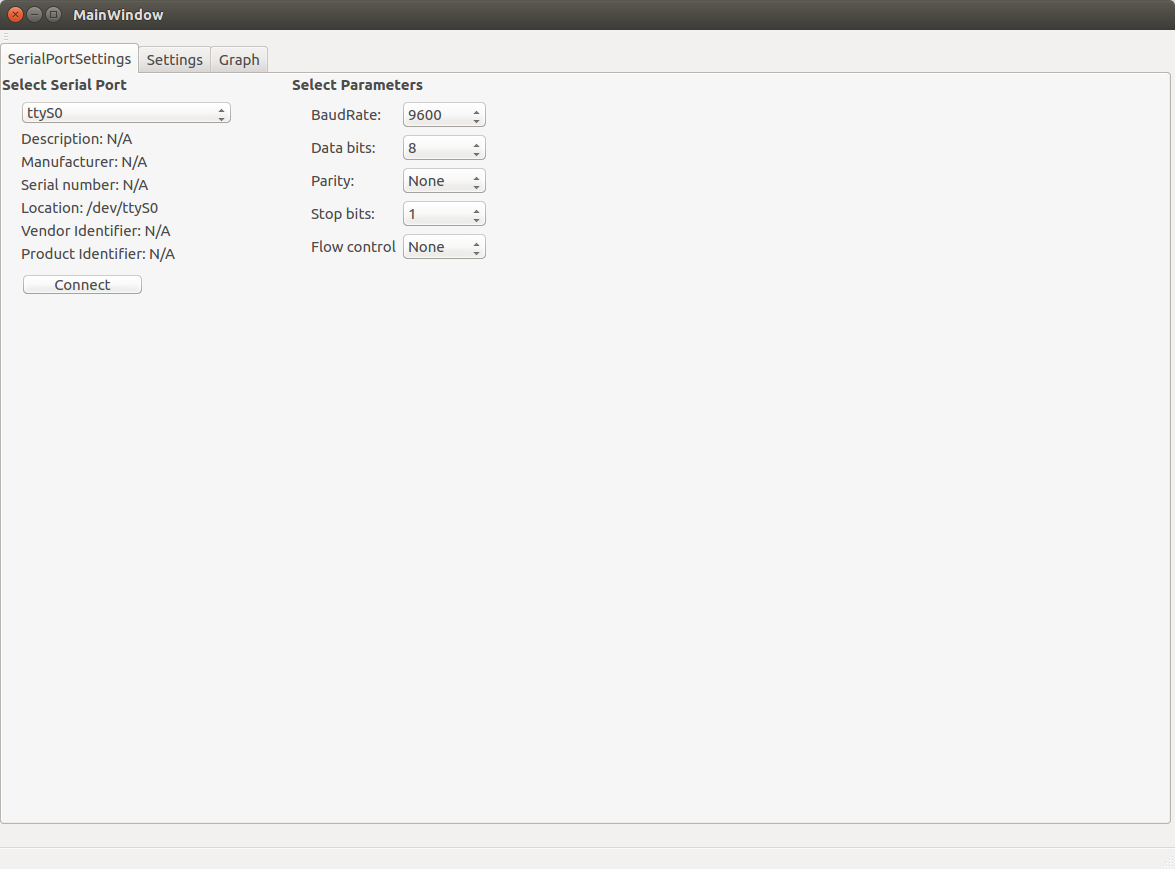
\includegraphics[scale=0.4]{Pictures/QuadroTune/QuadroTuneSerialSettings.png}
		%\rule{35em}{0.5pt}
	\caption[Aplikacja użytkownika do strojenia parametrów lotu - ustawienia portu szeregowego]{Aplikacja użytkownika do strojenia parametrów lotu - ustawienia portu szeregowego}
	\label{fig:QuadroTune_screen1}
\end{figure}

Rysunek ~\ref{fig:QuadroTune_screen1} przedstawia ekran służący do konfiguracji parametrów portu szeregowego. Z rozwijanej listy widocznej pod napisem ''Select serial port'' użytkownik wybiera moduł HC-06 znajdujący się na płytce kontrolera lotu kwadrokoptera. Po wciśnięciu przycisku ''Connect'' aplikacja rozpoczyna próbę nawiązania połączenia z kwadrokopterem informując użytkownika o przebiegu operacji za pomocą paska informacyjnego u dołu ekranu (w przypadku braku komunikatów pasek ten pozostaje pusty).

\begin{figure}[H]
	\centering
	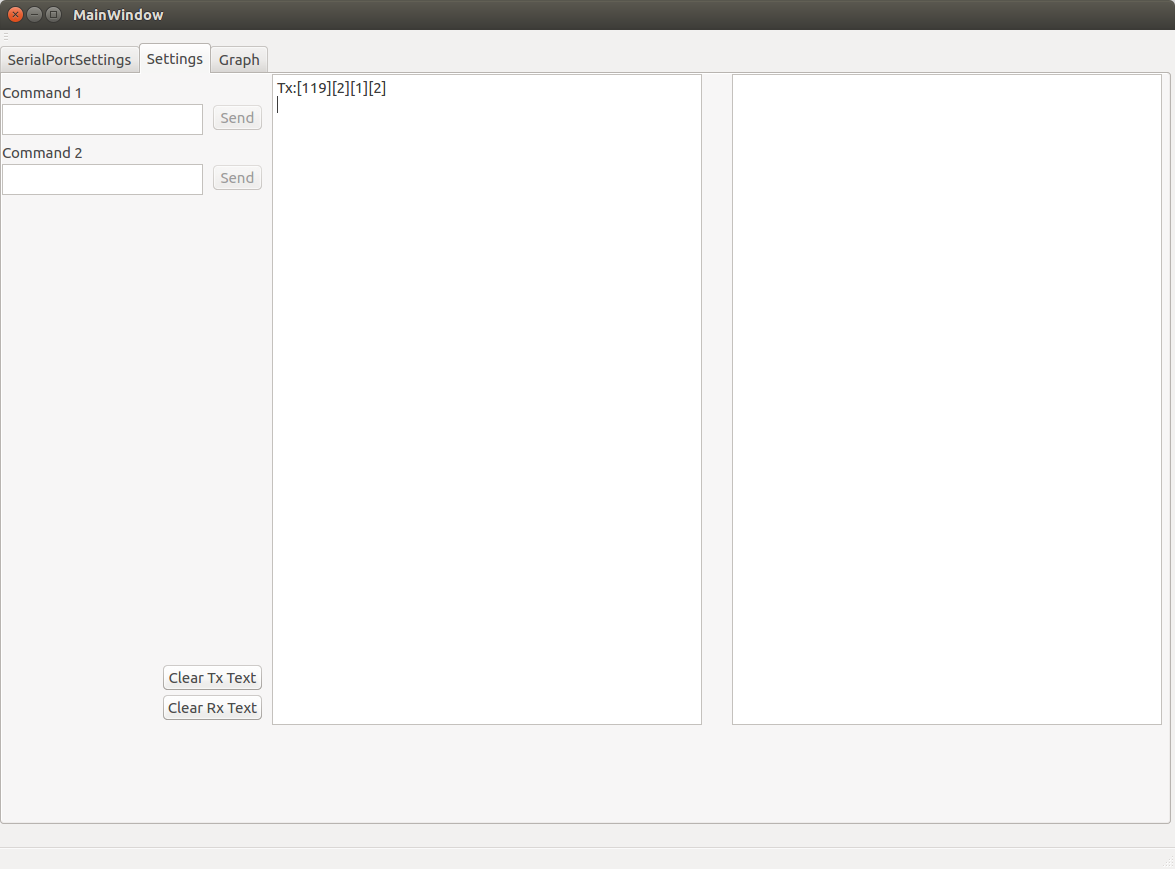
\includegraphics[scale=0.4]{Pictures/QuadroTune/QuadroTuneSettings.png}
		%\rule{35em}{0.5pt}
	\caption[Aplikacja użytkownika do strojenia parametrów lotu - ustawienia rejestrów kwadrokoptera]{Aplikacja użytkownika do strojenia parametrów lotu - ustawienia rejestrów kwadrokoptera}
	\label{fig:QuadroTune_screen2}
\end{figure}

Rysunek ~\ref{fig:QuadroTune_screen2} przedstawia okno służące do zapisu rejestrów wewnętrznych kwadrokoptera. W lewej części okna widać dwa pola opisane jako ''Command1'' oraz ''Command2'', w których użytkownik wpisuje komendy jakie mają zostać wysłane. Komendy powinny być wpisywane zgodnie z omówionym wcześniej protokołem, używanym do komunikacji z kwadrokopterem, jednakże dla wygody uzytkowania wszystkie pola ramki uzupełnia się w trybie tekstowym, a aplikacja przetwarza tę postać na wartości binarne. Dla przykładu, gdy użytkownik chce zapisać trzy rejestry wewnętrzne kwadrokoptera począwszy od rejestru o adresie 1 wartościami 156, 10 i 250 musi on wpisać w polę ''Command1'' lub ''Command2'' następujący ciąg znaków:

w,1,3,156,10,250

gdzie:
\begin{itemize}
	\item w - oznacza komendę zapisu rejestrów.
	\item 1 - oznacza adres pierwszego zapisywanego rejestru.
	\item 3 - oznacza liczbę zapisywanych rejestrów.
	\item 156 - oznacza wartość pierwszego zapisywanego rejestru.
	\item 10 - oznacza wartość drugiego zapisywanego rejestru.
	\item 250 - oznacza wartość trzeciego zapisywanego rejestru.
\end{itemize}
Poszczególne pola wiadomości oddzielone są przecinkiem.

Analogicznie przy chęci odczytu 5 rejestrów począwszy od rejestru o adresie 7 użytkownik powinien wpisać nastepującą komendę:

r,2,7,5

gdzie:
\begin{itemize}
	\item r - oznacza komendę odczytu rejestrów.
	\item 2 - oznacza długość pola danych wiadomości w bajtach.
	\item 7 - oznacza adres pierwszego rejestru do odczytu.
	\item 5 - oznacza liczbę rejestrów do odczytu.
\end{itemize}
Dane wysyłane przez użytkownika w stronę kwadrokoptera pokazują się w oknie po lewej stronie ekranu, natomiast dane wysłane przez kwadrokopter  otrzymane przez aplikacje w oknie po prawej stronie ekranu. Przyciski ''Clear Tx Text'' oraz ''Clear Rx Text'' służą do czyszczenia tekstu odpowiednio w lewym i prawym oknie wiadomości. 

\begin{figure}[H]
	\centering
	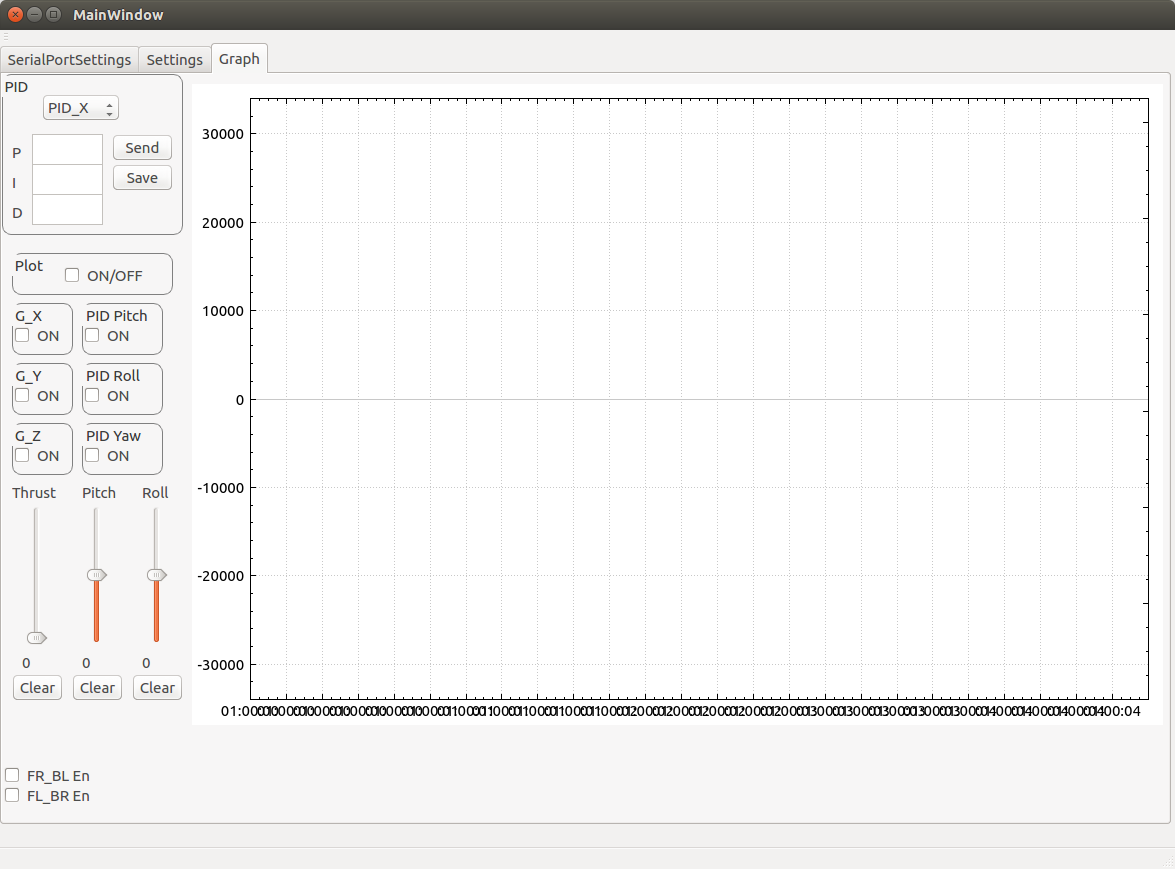
\includegraphics[scale=0.4]{Pictures/QuadroTune/QuadroTuneGraph.png}
		%\rule{35em}{0.5pt}
	\caption[Aplikacja użytkownika do strojenia parametrów lotu - ustawienia regulatorów PID]{Aplikacja użytkownika do strojenia parametrów lotu - ustawienia regulatorów PID}
	\label{fig:QuadroTune_screen3}
\end{figure}

Rysunek ~\ref{fig:QuadroTune_screen3} przedstawia główne okno służące do strojenia regulatorów PID używanych przez algorytm stabilizacji lotu oraz do przedstawiania odczytów z żyroskopu umieszczonego w kwadrokopterze, jak również wartości wyjściowych z regulatorów PID w postaci graficznej.

W lewym górnym rogu okna widać pole wyboru nastawianego w danej chwili regulatora PID. Po wybraniu jednej z trzech możliwych wartości (PID\_X, PID\_Y, PID\_Z) aplikacja odczytuje wartości członów P, I oraz D wybranego regulatora z pamięci kwadrokoptera. Następnie po modyfikacji parametrów regulatora następuje wysłanie nowych nastaw przez wciśnięcie przycisku ''Send''. Przycisk ''Save'' powoduje wysłanie do kwadrokoptera komendy zapisującej obecne nastawy wszystkich regulatorów PID w pamięci EEPROM kontrolera lotu. Poniżej części odpowiedzialnej za konfigurację regulatorów PID, znajdują się pola służące do włączania i wyłączania całego wykresu oraz do wybierania, które jego składniki (wartości pomairów żyroskopu, wartości wyjściowe regulatorów PID) mają być widoczne dla użytkownika. Poniżej widać trzy suwaki, służące do płynnej zmiany zadanej wartości ciągu silników oraz prędkości przechylenia i wychylenia. Są one używane do testów i ustawiania parametrów regulatorów PID odpowiedzialnych za obrót kwadrokoptera wokół osi X i Y. 


\section{Interfejs użytkownika do kontroli lotu}

Podobnie jak w przypadku aplikacji służącej to ustawiania parametrów lotu kwadrokoptera, aplikacja przeznaczona służąca do kontroli kwadrokoptera nie jest przedmiotem niniejszej pracy dyplomowej, dlatego też omówione zostanie jej działanie, a nie sama implementacja.

Omawiana aplikacja służy jedynie do kontroli kwadrokoptera w trakcie lotu. W związku z tym musi spełniać dwa podstawowe zadania:
\begin{itemize}
	\item Ustanowienie połączenia radiowego z kwadrokopterem.
	\item Przesyłanie do kwadrokoptera sygnałów sterujących jego lotem.
\end{itemize}

Obsługa aplikacji jest bardzo prosta. Użytkownik po jej włączeniu zostaje poproszony o możliwość włączenia modułu Bluetooth, w który wyposażony jest telefon. Następnie z listy urządzeń Bluetooth widzianych przez telefon, użytkownik wybiera moduł HC-06 umieszczony w płytce kontrolera lotu. Po wybraniu odpowiedniego urządzenia użytkownik uruchamia ekran odpowiedzialny za kontrolę kwadrokoptera, co inicjalizuje próbę nawiązania połączenia z kwadrokopterem. Gdy połączenie się powiedzie, użytkownik rozpoczyna sterowanie kwadrokopterem za pomocą dwóch joysticków wyświetlonych na ekranie telefonu.

\begin{figure}[H]
	\centering
	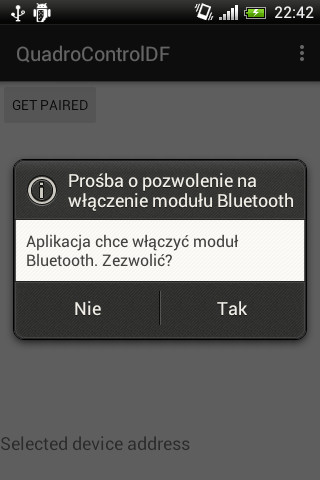
\includegraphics[scale=0.6]{Pictures/DroidAtScreen/droid@screen-1.png}
		%\rule{35em}{0.5pt}
	\caption[Aplikacja użytkownika - ekran startory]{Aplikacja użytkownika - ekran startowy}
	\label{fig:QuadroControl_screen1}
\end{figure}

Rysunek ~\ref{fig:QuadroControl_screen1} przedstawia wygląd komunikatu ukazującego się użytkownikowi zaraz po włączeniu aplikacji. W przypadku braku zgody na włączenie modułu Bluetooth aplikacja zostanie zamknięta.

\begin{figure}[H]
	\centering
	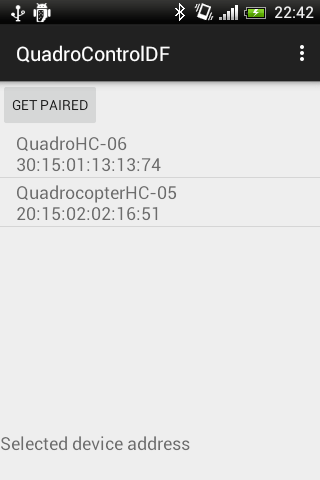
\includegraphics[scale=0.6]{Pictures/DroidAtScreen/droid@screen-2.png}
		%\rule{35em}{0.5pt}
	\caption[Aplikacja użytkownika - parowanie urządzeń]{Aplikacja użytkownika - parowanie urządzeń}
	\label{fig:QuadroControl_screen2}
\end{figure}

Rysunek ~\ref{fig:QuadroControl_screen2} przedstawia ekran widoczny po wyrażeniu zgody na włączenie modułu Bluetooth wewnątrz telefonu. Aplikacja pobiera listę urządzeń, które są widoczne dla telefonu i przedstawia ich nazwy wraz z unikalnymi identyfikatorami. 

\begin{figure}[H]
	\centering
	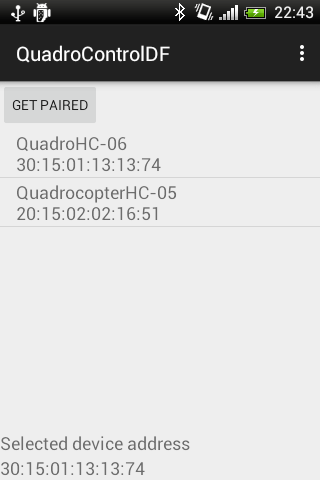
\includegraphics[scale=0.6]{Pictures/DroidAtScreen/droid@screen-3.png}
		%\rule{35em}{0.5pt}
	\caption[Aplikacja użytkownika - Ekran startory]{Aplikacja użytkownika - Wybór urządzenia}
	\label{fig:QuadroControl_screen3}
\end{figure}

Rysunek ~\ref{fig:QuadroControl_screen3} przedstawia wygląd głównego okna aplikacji po wyborze modułu Bluetooth umieszczonego w płytce kwadrokopterze. Identyfikator wybranego urządzenia pojawił się w dolnej części ekranu. Z tego miejsca użytkownik może przejść do ekranu, za pomocą którego możliwa jest kontrola lotu kwadrokoptera.

\begin{figure}[H]
	\centering
	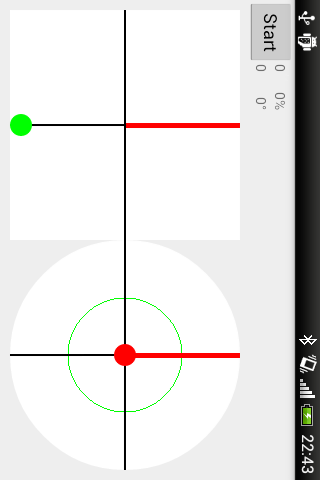
\includegraphics[scale=0.8, angle=90]{Pictures/DroidAtScreen/droid@screen-4.png}
		%\rule{35em}{0.5pt}
	\caption[Aplikacja użytkownika - ekran kontroli]{Aplikacja użytkownika - ekran kontroli}
	\label{fig:QuadroControl_screen4}
\end{figure}

Rysunek ~\ref{fig:QuadroControl_screen4} przedstawia ekran służący do kontroli lotu kwadrokoptera. Widoczne są na nim dwa joysticki, z czego joystick widoczny po lewej stronie odpowiedzialny jest za kontrolę ciągu silników (ruch joysticka góra - dół) oraz za obrót kwadrokoptera wokół osi Z (ruch joysticka lewo-prawo), natomiast joystick widoczny po prawej stronie odpowiedzialny jest za przechylenie (ruch joysticka lewo-prawo) oraz pochylenie (ruch joysticka góra-dół). W lewym górnym rogu ekranu widać przycisk ''Start'' służący do rozpoczęcia lotu kwadrokoptera oraz cztery pola wyświetlające wartości liczbowe informujące o położeniu w pionie i poziomie każdego z joyskicków, służące do celów testowych.

